\documentclass[11pt,spanish]{article}
\usepackage[spanish]{babel}
\selectlanguage{spanish}
\usepackage[utf8]{inputenc}
\usepackage{graphicx}
\usepackage{caption}
\usepackage{subcaption}
\usepackage{hyperref}
\usepackage[top=1in, bottom=1.25in, left=1.25in, right=1in]{geometry}

\begin{document}

\title{Redes Neuronales Profundas: Trabajo Práctico 2}
\date{}
\maketitle

\section*{Respuestas}
El código realizado para la resolución de los ejercicios está disponible en \href{https://github.com/dncampo/deep-learning/tree/lpineda}{github} (branch \textit{lpineda})

\subsection*{Ejercicio 1}
El ejercicio tutorial propuesto consiste en definir una función $f(x,y) = x^2+2xy+y^2$ en Theano. La única modificación debe realizarse en la variable ``out''. \par

Para el ejemplo de regresion lineal, se separa el dataset en mini-batches para ir entrenando el modelo de forma progresiva, utilizando subconjuntos de datos. 
Con el dataset de motos y aviones de Caltech101, las imagenes son leidas y apiladas como vectores en una matriz que representa el dataset, y cada clase se representa con un vector de 0 o un 1. Luego el entrenamiento se realiza por épocas, finalizando cuando el error de entrenamiento no varia más que cierto umbral en las últimas 50 épocas o por máximo de iteraciones. La evolución del error de entrenamiento y test se puede observar en la figura \ref{ex1b2}
\begin{figure}[htbp]
	\centering
	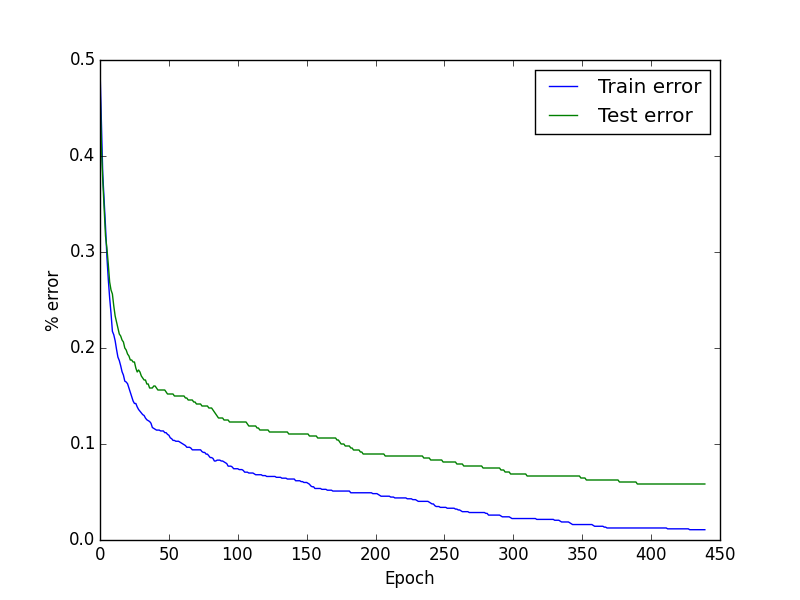
\includegraphics[width=0.5\textwidth]{../ex1b2.png}
	\caption{Error de train y test}
	\label{ex1b2}
\end{figure}

Finalmente, para la tercera parte de este ejercicio se debe agregar al model una capa oculta de 100 neuronas con activación ReLU. Para esto es necesario definir una nueva matriz de pesos y un nuevo vector de bias para esta capa oculta. Además, se debe modificar la función de actualización para que calcule los delta usando los gradientes de la capa oculta. El entrenamiento se realiza de la misma manera que en el ejemplo de regresión lineal. La evolución del error de entrenamiento y test se puede observar en la figura \ref{ex1b3}

\begin{figure}[htbp]
	\centering
	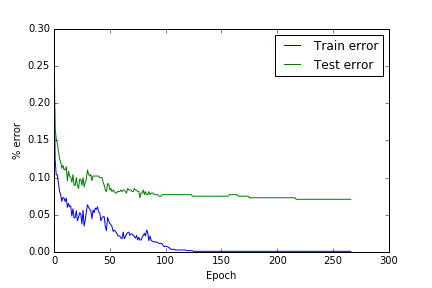
\includegraphics[width=0.5\textwidth]{../ex1b3.png}
	\caption{Error de train y test de modelo con capa oculta de 100 neuronas}
	\label{ex1b3}
\end{figure}


\subsection*{Ejercicio 2}

En la figura \ref{fig:keras_example_history} se muestra la evolución del entrenamiento de la red neuronal con el dataset completo de $60000$ ejemplos.
El modelo está compuesto por dos capas de 512 neuronas, un dropout de $0.2$ y activación ReLU, y una capa de salida de 10 neuronas y activación softmax.

\begin{figure}[htpb]
\centering
\begin{minipage}{.5\textwidth}
  \centering
  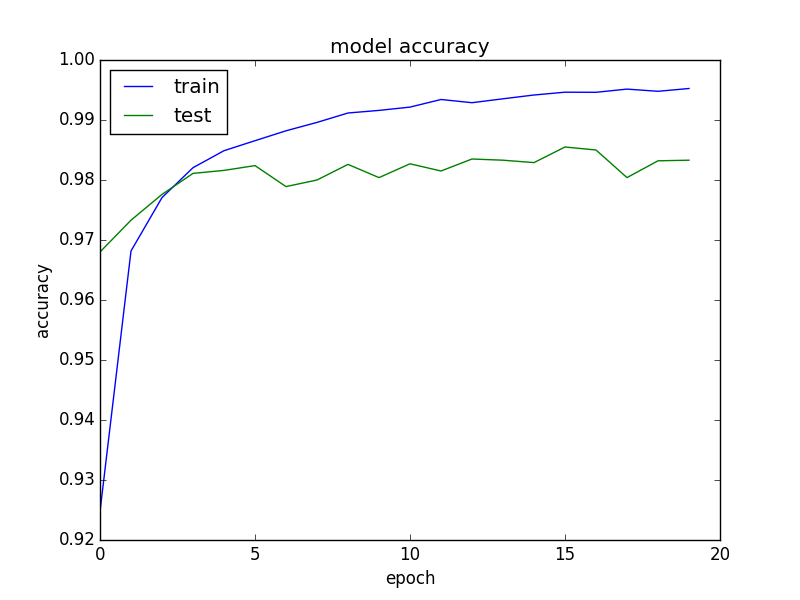
\includegraphics[width=1\linewidth]{../keras_example_acc.png}
\end{minipage}%
\begin{minipage}{.5\textwidth}
  \centering
  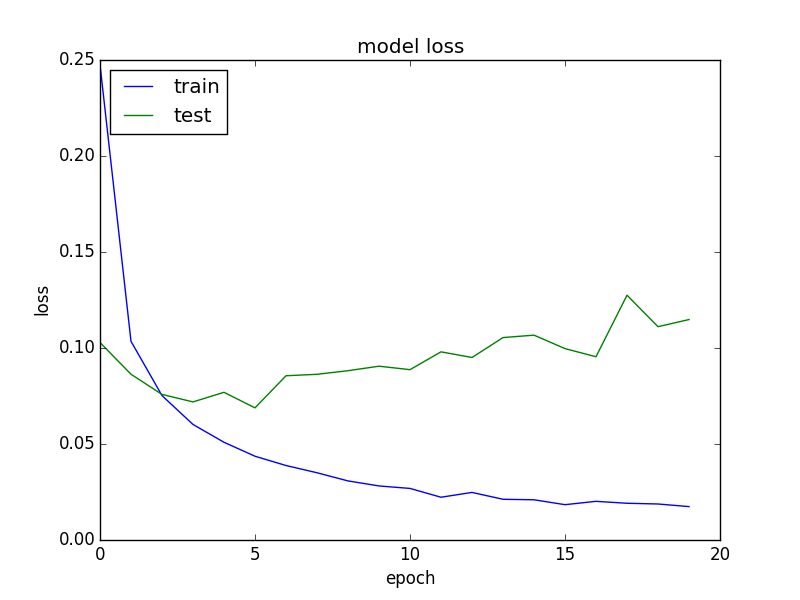
\includegraphics[width=1\linewidth]{../keras_example_loss.png}
\end{minipage}
\caption{Ejemplo de Redes Neuronales de Keras con todos los patrones}
\label{fig:keras_example_history}
\end{figure}

En la figura \ref{fig:ex2a1} se muestra la evolución del entrenamiento de la red neuronal con el 25\% de los ejemplos del dataset y la misma red neuronal. En este caso la precisión del model bajo un 2\% respecto del entrenado con el dataset completo. \par

\begin{figure}[tpb]
\centering
\begin{minipage}{.5\textwidth}
  \centering
  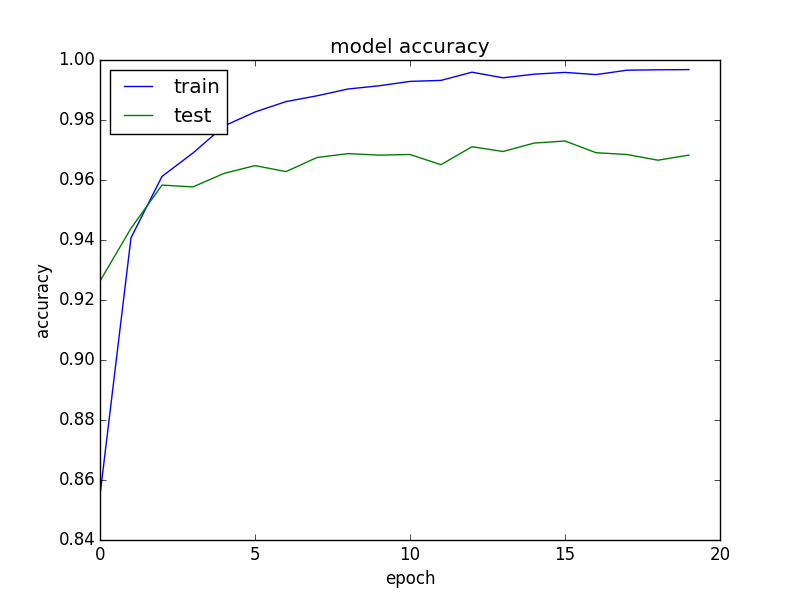
\includegraphics[width=1\linewidth]{../ex2a1_acc.png}
\end{minipage}%
\begin{minipage}{.5\textwidth}
  \centering
  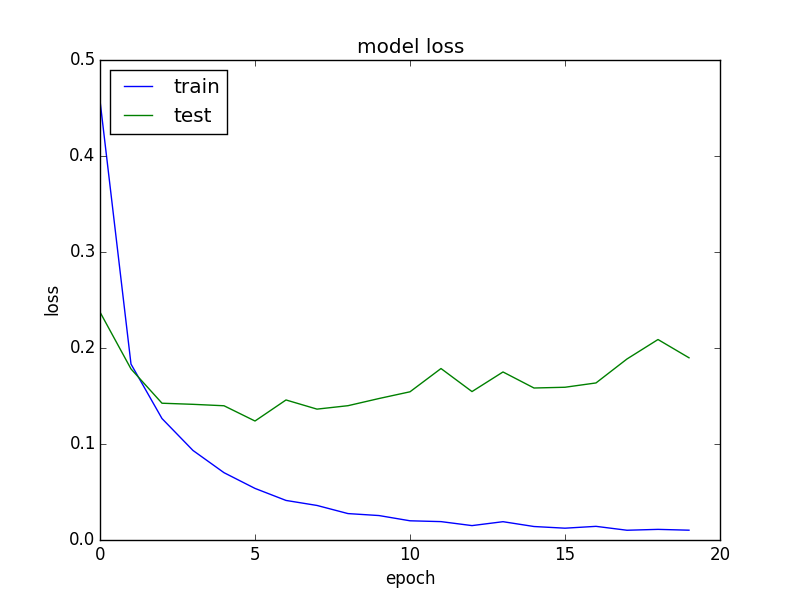
\includegraphics[width=1\linewidth]{../ex2a1_loss.png}
\end{minipage}
\caption{Utilizando el 25\% de los datos para entrenamiento}
\label{fig:ex2a1}
\end{figure}

En la figura \ref{fig:ex2a2} se muestra la evolución del entrenamiento de la red neuronal con el 25\% de los ejemplos del dataset y una red neuronal con una sola capa de 512 neuronas con activación ReLU y dropout de $0.2$. 

\begin{figure}[tpb]
\centering
\begin{minipage}{.5\textwidth}
  \centering
  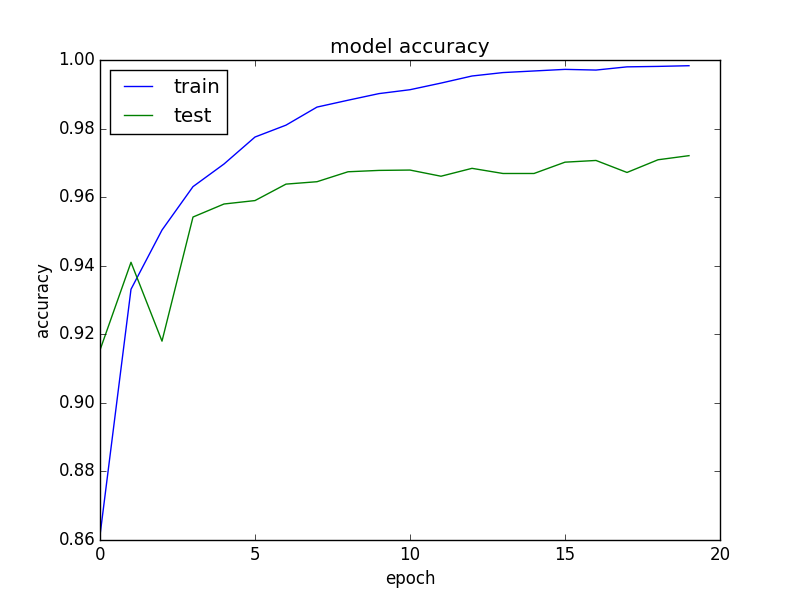
\includegraphics[width=1\linewidth]{../ex2a2_acc.png}
\end{minipage}%
\begin{minipage}{.5\textwidth}
  \centering
  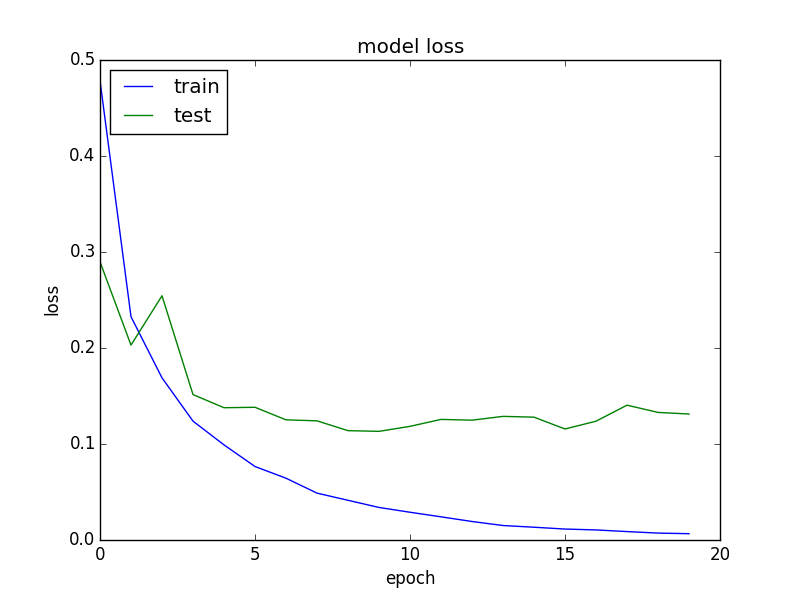
\includegraphics[width=1\linewidth]{../ex2a2_loss.png}
\end{minipage}
\caption{Utilizando solo una capa con activación ReLU}
\label{fig:ex2a2}
\end{figure}

En la figura \ref{fig:ex2a3} se muestra la evolución del entrenamiento de la red neuronal con el 25\% de los ejemplos del dataset y una red neuronal con una sola capa de 512 neuronas con activación sigmoidea y dropout de $0.2$. 

\begin{figure}[tpb]
\centering
\begin{minipage}{.5\textwidth}
  \centering
  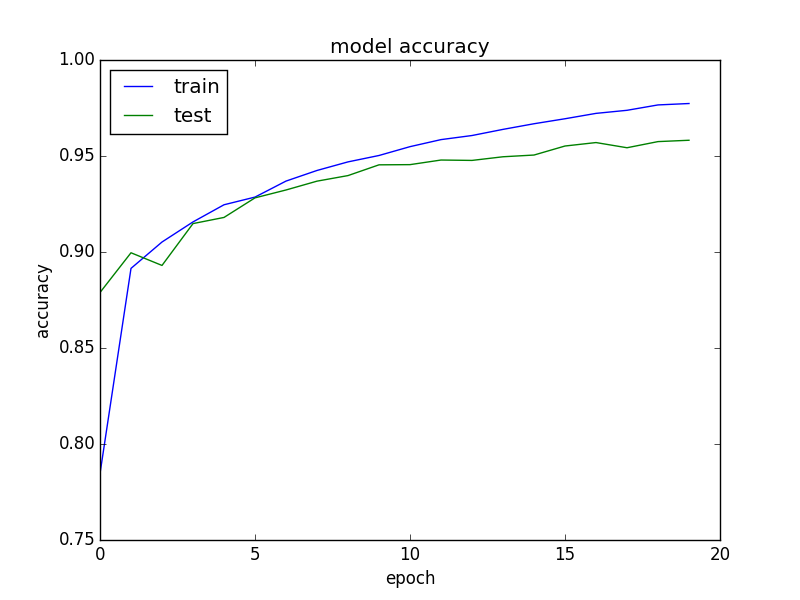
\includegraphics[width=1\linewidth]{../ex2a3_acc.png}
\end{minipage}%
\begin{minipage}{.5\textwidth}
  \centering
  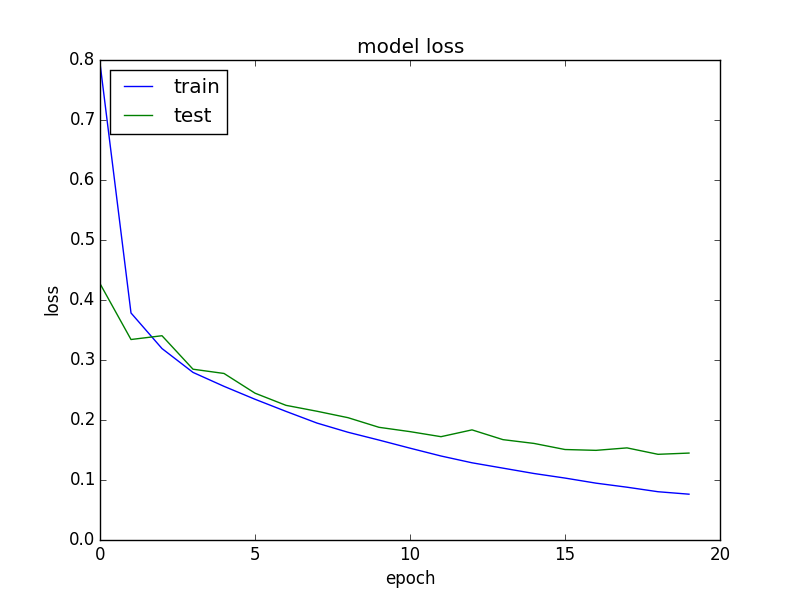
\includegraphics[width=1\linewidth]{../ex2a3_loss.png}
\end{minipage}
\caption{Utilizando solo una capa con activación sigmoidea}
\label{fig:ex2a3}
\end{figure}

En la figura \ref{fig:ex2a4} se muestra la evolución del entrenamiento de la red neuronal con el 25\% de los ejemplos del dataset y una red neuronal con una sola capa de 512 neuronas con activación sigmoidea y dropout de $0.5$. 


\begin{figure}[tpb]
\centering
\begin{minipage}{.5\textwidth}
  \centering
  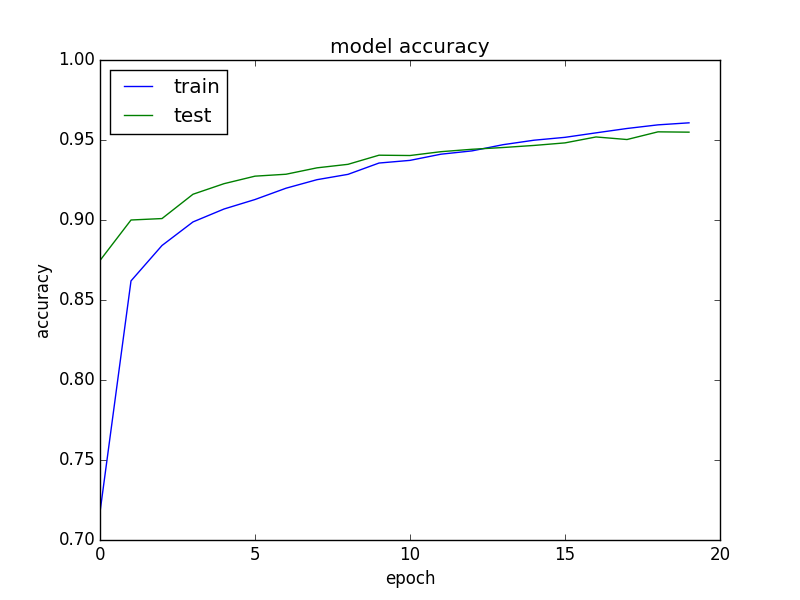
\includegraphics[width=1\linewidth]{../ex2a4_acc.png}
\end{minipage}%
\begin{minipage}{.5\textwidth}
  \centering
  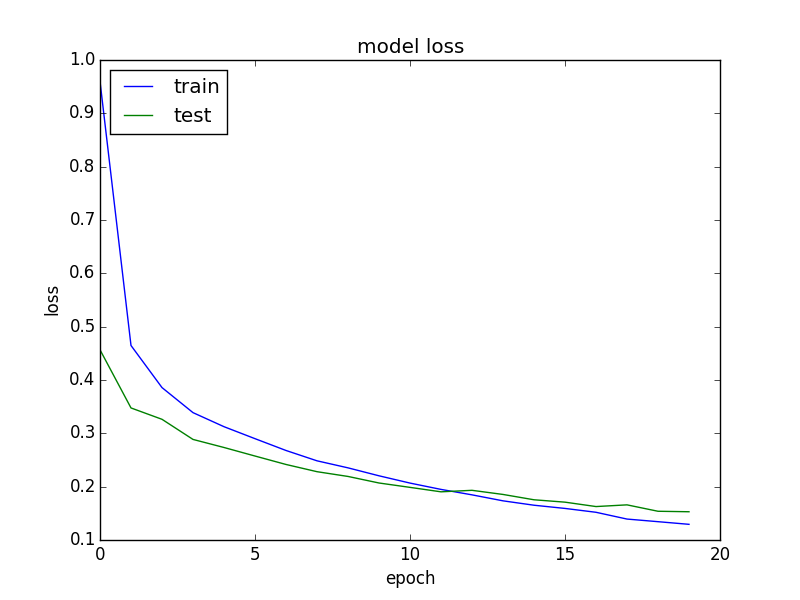
\includegraphics[width=1\linewidth]{../ex2a4_loss.png}
\end{minipage}
\caption{Utilizando solo una capa con activación sigmoidea y dropout de 0.5}
\label{fig:ex2a4}
\end{figure}

En la figura \ref{fig:ex2a5} se muestra la evolución del entrenamiento de la red neuronal con el 25\% de los ejemplos del dataset y una red neuronal con una sola capa de 512 neuronas con activación sigmoidea. 

\begin{figure}[tpb]
\centering
\begin{minipage}{.5\textwidth}
  \centering
  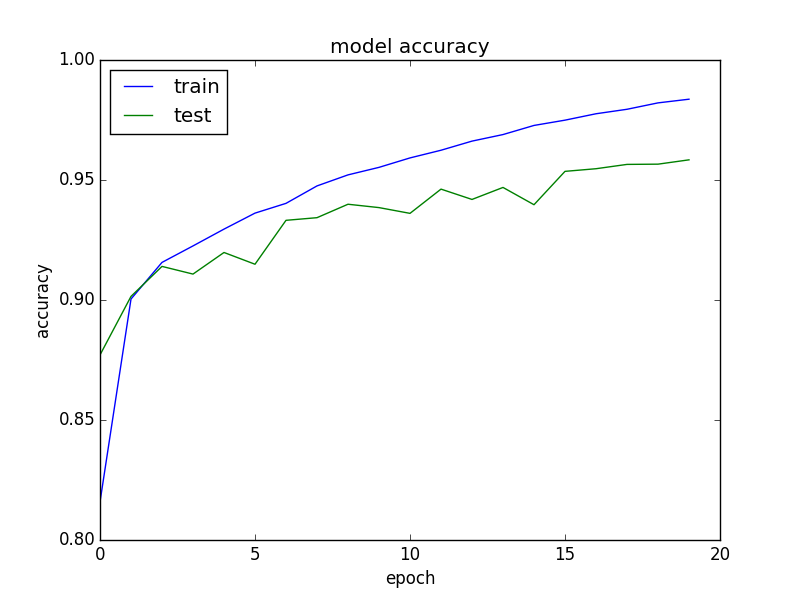
\includegraphics[width=1\linewidth]{../ex2a5_acc.png}
\end{minipage}%
\begin{minipage}{.5\textwidth}
  \centering
  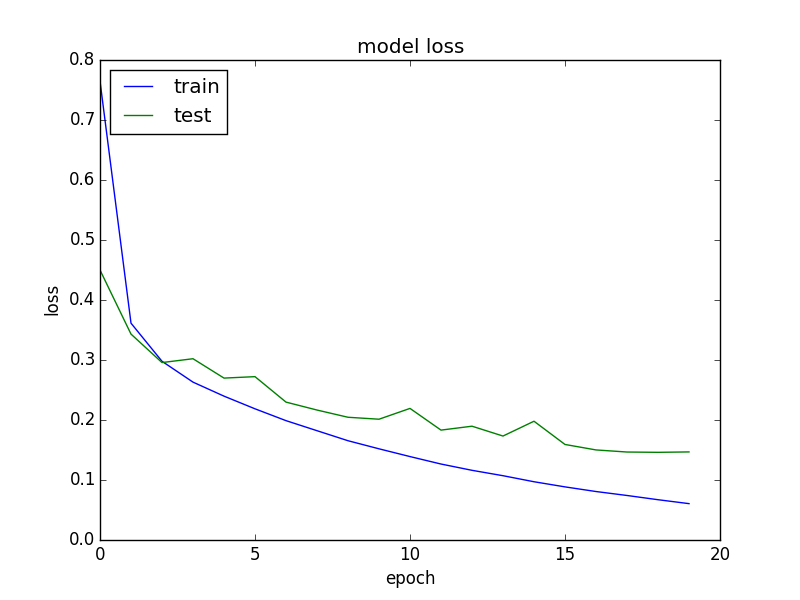
\includegraphics[width=1\linewidth]{../ex2a5_loss.png}
\end{minipage}
\caption{Utilizando solo una capa con activación sigmoidea pero sin dropout}
\label{fig:ex2a5}
\end{figure}

\paragraph{Trabajo práctico 1} Las funciones del ejercicio (b) implementadas con primitivas de Keras pueden encontrarse en el repositorio GitHub.

Finalmente, el formato h5 permite salvar el modelo entrenado usando un formato que soporta una cantidad ilimitada de tipos de datos. De esta forma, podemos distribuir en un archivo un modelo entrenado, sin necesidad de recalcularlo, o guardar modelos intermedios en las distintas épocas de entrenamiento.
\end{document}
